\chapter{Parallel Implementation}
 \label{chap:pi}
 \section{Introduction}
\hspace{10mm}In the parallel implementation the unique NEC numbering, CVS generation in data graph, and checking whether the query graph exists in the sub-graph and the combination generation are done in GPU.

\section{Algorithm}
 \label{sec:al}
 
\begin{breakablealgorithm}[H]
\caption{Parallel $Turbo_{iso}$}
%\label{Graph Isomorphism}
\textbf{Procedure}: NECGen()\\
Parallel NEC generation on each node.\\
\textbf{Input}: Query Graph $Q$.\\
\textbf{Output}: NEC.\\
\begin{algorithmic}
\item \begin{enumerate}
\item repeat until all nodes got NEC
\item Run parallel on all nodes
\begin{enumerate}
\item running on node v
\item iterate over all neighbors of vertex v
\item \hspace{10mm}if not all neighbors have NEC return
\item find the hash of neighborhood.set its hash location to 1.
\end{enumerate}
\item assign unique numbering to all 1's in the hash array
\item Run parallel on all nodes
\begin{enumerate}
\item running on node v
\item iterate over all neighbors of vertex v
\item \hspace{10mm}if not all neighbors have NEC return
\item find the hash of neighborhood.Find the unique NEC in hash location
\item assign it to the vertex
\end{enumerate}
\end{enumerate}
\end{algorithmic}
\textbf{Procedure}: CVSGen()\\
Parallel CVS generation for each NEC.\\
\textbf{Input}: Data Graph $Q$,NEC.\\
\textbf{Output}: CVS.\\
\begin{algorithmic}
\item \begin{enumerate}
\item all nodes in data graph is in NEC 1
\item for each NEC from 2 to last
\item Run parallel on all nodes
\begin{enumerate}
\item running on node v
\item iterate over all neighbors of vertex v.
\item \hspace{10mm}check the existence of the neighborhood of NEC on the node v.
\item \hspace{10mm}if found set the flag 1.
\end{enumerate}
\end{enumerate}
\end{algorithmic}
\textbf{Procedure}: PermandComb()\\
Parallelly check all possible permutations and combinations.\\
\textbf{Input}: Data Graph $D$, Query Graph $Q$, Current vertex index(i),Possibilities(P),Maximum Possibilities(MP)\\
\textbf{Output}: Mapping of nodes from query graph to data graph.\\
\begin{algorithmic}
\item \begin{enumerate}
\item if i= $|V(q)|$
\item \hspace{10mm}Report all values in P and return
\item else
 \begin{enumerate}
\item find u,the NEC of the vertex
\item Multiply P with CVSGen(u)
\item while $P >= MP$
 \begin{enumerate}
\item call CheckMap() on MP elements of P
\item call Exclusive-scan on Checkmap output
\item Save valid possibilities to newP 
\item P-=MP (numbers)
\end{enumerate}
\item move newP to P.
\end{enumerate}
\end{enumerate}
\end{algorithmic}
\textbf{Procedure}: CheckMap()\\
Parallel check of existence of query graph.\\
\textbf{Input}: Data Graph $D$,Map m,Query Graph $Q$,till vertex $v$ in query graph.\\
\textbf{Output}: true/false.\\
\begin{algorithmic}
\item \begin{enumerate}
\item running on all nodes u if $u<=v$.
\item iterate over all neighbors of vertex u.
\item \hspace{10mm}check the existence of all edges in data graph corresponding to one in query graph.
\item \hspace{10mm}if not all edges present set false.
\end{enumerate}

\end{algorithmic}
\end{breakablealgorithm}
\par The procedure $NECGen$ gives unique ids to one tree in the query graph similar to Figure 4. We do a level order traversal on the tree. So at some nodes all its children may not have NEC given we process those nodes in the next iterations. The step 2 finds the neighborhoods that can be processed at the current iteration and finds a hash of the neighborhood. To these unique hashes we assign numbering by SCAN algorithm. Then these numbering are assigned back to each nodes.
\par The procedure $CVSGen $ finds the candidates for a particular NEC. They check on each node on data graph and checks the neighboring nodes for matching neighbors of the particular NEC in query graph.
\par The procedure $PermandComb$ finds all possibilities of the query graph. For each vertex of query graph it finds all possibilities(current possibilities x CvsGen(u)). If the possibilities is more than we can store(MP), $CheckMap$ is called on all current possibilities and the wrong ones are removed. This will make the P $<$MP.  At last when i= $|V(q)|$,  P has all valid possibilities. The procedure $CheckMap$ checks the existence of non tree edges in the current 	mapping. If $CheckMap$ returns true it is reported as a correct mapping.
\begin{figure}[h!]
 \begin{minipage}{.3\textwidth}
 \centering
  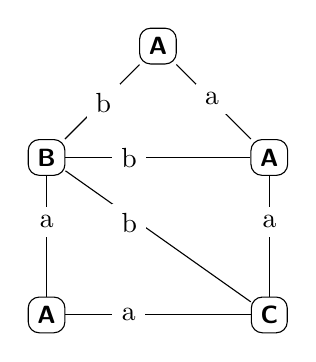
\begin{tikzpicture}[node distance=2cm,node/.style={rounded corners,draw,font=\sffamily\small\bfseries}]
	\node[node] (1) {A};
	\node[node] (2)[below left of=1] {B};
		\node[node] (3)[below right of=1] {A};
		\node[node] (4)[below  of=2] {A};
			\node[node] (5)[below of=3] {C};
	\path
	(1) edge node [minimum width = 1em, fill = white,pos=.25,below left] {b} (2)
		edge node [minimum width = 1em, fill = white,pos=.25,below right]{a} (3)	
	(2) edge node [minimum width = 1em, fill = white,pos=.25,right]{b} (3)
		edge node [minimum width = 1em, fill = white,pos=.25,below]{a} (4)
		edge node [minimum width = 1em, fill = white,pos=.25,below right]{b} (5)
	(3) edge node [minimum width = 1em, fill = white,pos=.25,below]{a} (5)	
	(4) edge node [minimum width = 1em, fill = white,pos=.25,right]{a} (5);	
							
\end{tikzpicture}
\\\textbf{Step 1}
\end{minipage}
 \begin{minipage}{.3\textwidth}
	 \centering
	 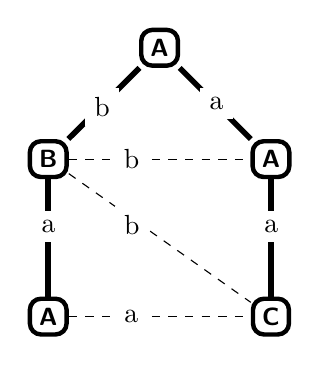
\begin{tikzpicture}[node distance=2cm,node/.style={rounded corners,draw,font=\sffamily\small\bfseries}]
	\node[node,line width=1.6pt] (1) {A};
	\node[node,line width=1.6pt] (2)[below left of=1] {B};
		\node[node,line width=1.6pt] (3)[below right of=1] {A};
		\node[node,line width=1.6pt] (4)[below  of=2] {A};
			\node[node,line width=1.6pt] (5)[below of=3] {C};
	\path
	(1) edge[line width=.7mm] node [minimum width = 1em, fill = white,pos=.25,below left] {b} (2)
		edge[line width=.7mm] node [minimum width = 1em, fill = white,pos=.25,below right]{a} (3)	
	(2) edge[dashed] node [minimum width = 1em, fill = white,pos=.25,right]{b} (3)
		edge[line width=.7mm] node [minimum width = 1em, fill = white,pos=.25,below]{a} (4)
		edge[dashed] node [minimum width = 1em, fill = white,pos=.25,below right]{b} (5)
	(3) edge[line width=.7mm] node [minimum width = 1em, fill = white,pos=.25,below]{a} (5)	
	(4) edge[dashed] node [minimum width = 1em, fill = white,pos=.25,right]{a} (5);	
							
\end{tikzpicture}
\\\textbf{Step 2}
\end{minipage}
\begin{minipage}{.3\textwidth}
	 \centering
	 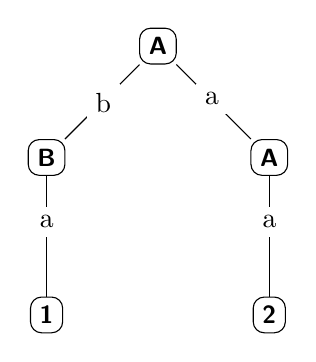
\begin{tikzpicture}[node distance=2cm,node/.style={rounded corners,draw,font=\sffamily\small\bfseries}]
	\node[node] (1) {A};
	\node[node] (2)[below left of=1] {B};
		\node[node] (3)[below right of=1] {A};
		\node[node] (4)[below  of=2] {1};
			\node[node] (5)[below of=3] {2};
	\path
	(1) edge[] node [minimum width = 1em, fill = white,pos=.25,below left] {b} (2)
		edge[] node [minimum width = 1em, fill = white,pos=.25,below right]{a} (3)	
	(2) edge[] node [minimum width = 1em, fill = white,pos=.25,below]{a} (4)
	(3) edge[] node [minimum width = 1em, fill = white,pos=.25,below]{a} (5);							
\end{tikzpicture}
\\\textbf{Step 3}
\end{minipage}\\
\vspace{5mm}
\begin{minipage}{.3\textwidth}
	 \centering
	 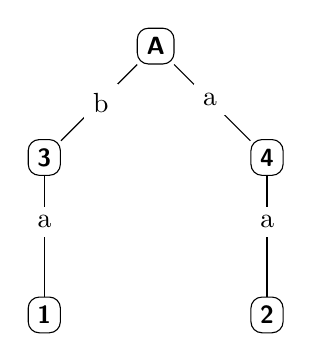
\begin{tikzpicture}[node distance=2cm,node/.style={rounded corners,draw,font=\sffamily\small\bfseries}]
	\node[node] (1) {A};
	\node[node] (2)[below left of=1] {3};
		\node[node] (3)[below right of=1] {4};
		\node[node] (4)[below  of=2] {1};
			\node[node] (5)[below of=3] {2};
	\path
	(1) edge[] node [minimum width = 1em, fill = white,pos=.25,below left] {b} (2)
		edge[] node [minimum width = 1em, fill = white,pos=.25,below right]{a} (3)	
	(2) edge[] node [minimum width = 1em, fill = white,pos=.25,below]{a} (4)
	(3) edge[] node [minimum width = 1em, fill = white,pos=.25,below]{a} (5);							
\end{tikzpicture}
\\\textbf{Step 4}
\end{minipage}
\begin{minipage}{.3\textwidth}
	 \centering
	 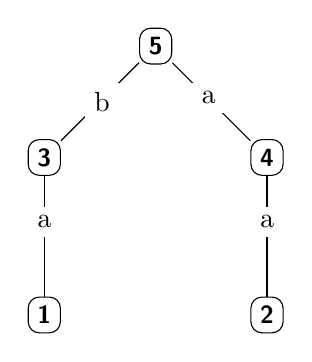
\begin{tikzpicture}[node distance=2cm,node/.style={rounded corners,draw,font=\sffamily\small\bfseries}]
	\node[node] (1) {5};
	\node[node] (2)[below left of=1] {3};
		\node[node] (3)[below right of=1] {4};
		\node[node] (4)[below  of=2] {1};
			\node[node] (5)[below of=3] {2};
	\path
	(1) edge[] node [minimum width = 1em, fill = white,pos=.25,below left] {b} (2)
		edge[] node [minimum width = 1em, fill = white,pos=.25,below right]{a} (3)	
	(2) edge[] node [minimum width = 1em, fill = white,pos=.25,below]{a} (4)
	(3) edge[] node [minimum width = 1em, fill = white,pos=.25,below]{a} (5);							
\end{tikzpicture}
\\\textbf{Step 5}
\end{minipage}
\begin{minipage}{.3\textwidth}
	 \centering
	 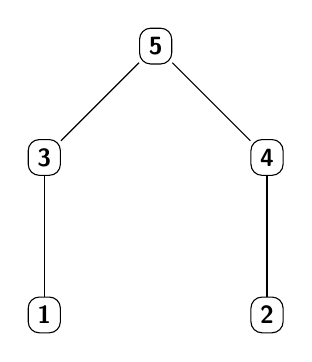
\begin{tikzpicture}[node distance=2cm,node/.style={rounded corners,draw,font=\sffamily\small\bfseries}]
	\node[node] (1) {5};
	\node[node] (2)[below left of=1] {3};
		\node[node] (3)[below right of=1] {4};
		\node[node] (4)[below  of=2] {1};
			\node[node] (5)[below of=3] {2};
	\path
	(1) edge[] node [] {} (2)
		edge[] node []{} (3)	
	(2) edge[] node []{} (4)
	(3) edge[] node []{} (5);							
\end{tikzpicture}
\\\textbf{Step 6}
\end{minipage}\\
\vspace{5mm}
\begin{minipage}{.3\textwidth}
\centering
\hfill \\

\begin{tikzpicture}[node distance=2cm,node/.style={rounded corners,draw,font=\sffamily\small\bfseries}]
\node[node,label=NEC 1] (2){A};
\end{tikzpicture}\\
\hfill \\

\begin{tikzpicture}[node distance=2cm,node/.style={rounded corners,draw,font=\sffamily\small\bfseries}]
\node[node,label=NEC 2] (2){C};
\end{tikzpicture}\\
\hfill \\
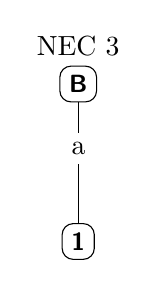
\begin{tikzpicture}[node distance=2cm,node/.style={rounded corners,draw,font=\sffamily\small\bfseries}]

\node[node,label=NEC 3] (2){B};
\node[node] (3)[below of=2]{1};
\path
	(2)	 edge node[minimum width = 1em, fill = white,pos=.25,below ] {a} (3);
\end{tikzpicture}
\end{minipage}
\begin{minipage}{.3\textwidth}
\centering
\hfill \\
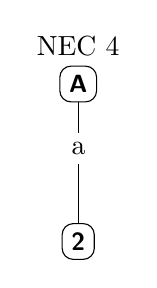
\begin{tikzpicture}[node distance=2cm,node/.style={rounded corners,draw,font=\sffamily\small\bfseries}]

\node[node,label=NEC 4] (2){A};
\node[node] (3)[below of=2]{2};
\path
	(2)	 edge node[minimum width = 1em, fill = white,pos=.25,below ] {a} (3);
\end{tikzpicture}
\hfill \\
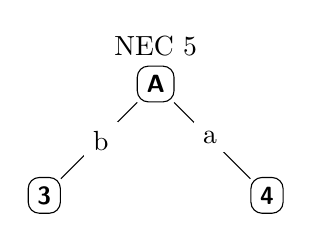
\begin{tikzpicture}[node distance=2cm,node/.style={rounded corners,draw,font=\sffamily\small\bfseries}]

\node[node,label=NEC 5] (2){A};
\node[node] (3)[below left of=2]{3};
\node[node] (4)[below right of=2]{4};
\path
	(2)	 edge node[minimum width = 1em, fill = white,pos=.25,below left] {b} (3)
		 edge node[minimum width = 1em, fill = white,pos=.25,below right] {a} (4);
\end{tikzpicture}
\\Classes
\end{minipage}
 \caption{Algorithm Query Graph Processing}
 \label{fig:working}
\end{figure}
 \par In the figure \ref{fig:working} the NEC's in query graph are detected. The first step is the finding of tree in the query graph. The bold lines in the image shows the selected tree in the query graph. In the next step the leaf nodes are given unique NEC's according to the node label. Then at each step the parent nodes whose all children has NEC defined, is given new NEC's. See the figure \ref{fig:working} and the NEC classes are given in the end. The NEC's are taking care of the edge labels so they are no longer required in the graph. 
\begin{figure}[h!]
\begin{minipage}{.4\textwidth}
	\centering
	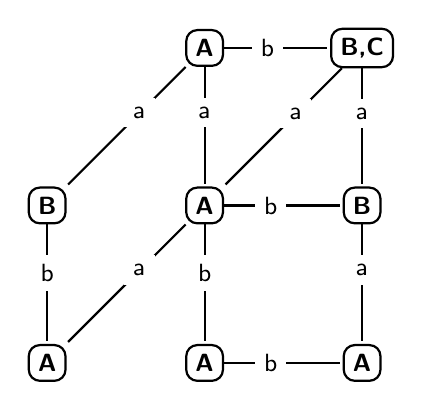
\begin{tikzpicture}[shorten >=1pt,auto,node distance=2cm,
                    thick,main node/.style={rounded corners,draw,font=\sffamily\small\bfseries}]

  \node[main node] (1) {A};
  \node[main node] (2) [right of=1] {B,C}; 
  \node[main node] (4) [below of =1] {A};
  \node[main node] (3) [left of=4] {B};
     \node[main node] (5) [below of=2] {B};
    \node[main node] (6) [below of=3] {A};
    \node[main node] (7) [below of=4] {A};
\node[main node] (8) [below of=5] {A};
  \path[every node/.style={font=\sffamily\small}]
    (1) edge[] node [minimum width = 1em, fill = white,pos=.25,right] {b} (2)
        edge[] node[minimum width = 1em, fill = white,pos=.25,below left] {a} (3)
        edge[] node[minimum width = 1em, fill = white,pos=.25,below] {a} (4)
    (2) edge[] node [minimum width = 1em, fill = white,pos=.25,below left] {a} (4)
        edge node [minimum width = 1em, fill = white,pos=.25,below] {a} (5)
    (3) edge[] node [minimum width = 1em, fill = white,pos=.25,below] {b} (6)
    (4) edge node [minimum width = 1em, fill = white,pos=.25,below] {b} (7)
    	edge[] node [minimum width = 1em, fill = white,pos=.25,below left] {a} (6) 
    	edge node [minimum width = 1em, fill = white,pos=.25,right] {b} (5) 
    (5) edge node [minimum width = 1em, fill = white,pos=.25,below] {a} (8)
    (7) edge node [minimum width = 1em, fill = white,pos=.25,right] {b} (8);	   
\end{tikzpicture}
\\\textbf{Step 1}
\end{minipage}
\begin{minipage}{.4\textwidth}
	\centering
	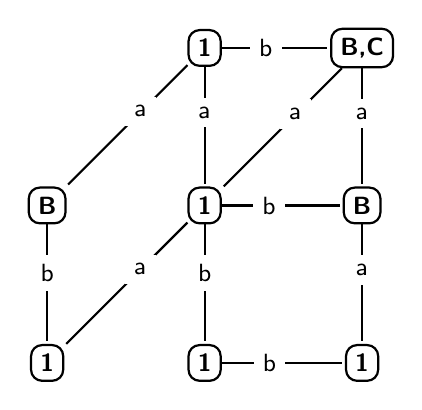
\begin{tikzpicture}[shorten >=1pt,auto,node distance=2cm,
                    thick,main node/.style={rounded corners,draw,font=\sffamily\small\bfseries}]

  \node[main node] (1) {1};
  \node[main node] (2) [right of=1] {B,C}; 
  \node[main node] (4) [below of =1] {1};
  \node[main node] (3) [left of=4] {B};
     \node[main node] (5) [below of=2] {B};
    \node[main node] (6) [below of=3] {1};
    \node[main node] (7) [below of=4] {1};
\node[main node] (8) [below of=5] {1};
  \path[every node/.style={font=\sffamily\small}]
    (1) edge[] node [minimum width = 1em, fill = white,pos=.25,right] {b} (2)
        edge[] node[minimum width = 1em, fill = white,pos=.25,below left] {a} (3)
        edge[] node[minimum width = 1em, fill = white,pos=.25,below] {a} (4)
    (2) edge[] node [minimum width = 1em, fill = white,pos=.25,below left] {a} (4)
        edge node [minimum width = 1em, fill = white,pos=.25,below] {a} (5)
    (3) edge[] node [minimum width = 1em, fill = white,pos=.25,below] {b} (6)
    (4) edge node [minimum width = 1em, fill = white,pos=.25,below] {b} (7)
    	edge[] node [minimum width = 1em, fill = white,pos=.25,below left] {a} (6) 
    	edge node [minimum width = 1em, fill = white,pos=.25,right] {b} (5) 
    (5) edge node [minimum width = 1em, fill = white,pos=.25,below] {a} (8)
    (7) edge node [minimum width = 1em, fill = white,pos=.25,right] {b} (8);	   
\end{tikzpicture}
\\\textbf{Step 2}
\end{minipage}\\
\hfill\vspace{5mm} \hfill\\
\begin{minipage}{.4\textwidth}
	\centering
	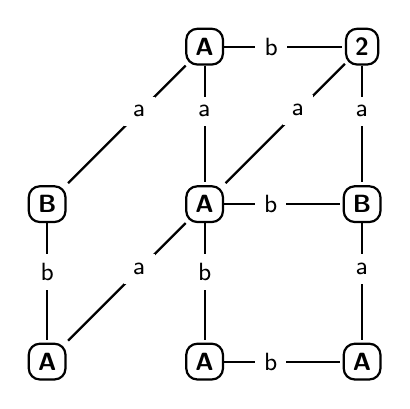
\begin{tikzpicture}[shorten >=1pt,auto,node distance=2cm,
                    thick,main node/.style={rounded corners,draw,font=\sffamily\small\bfseries}]

  \node[main node] (1) {A};
  \node[main node] (2) [right of=1] {2}; 
  \node[main node] (4) [below of =1] {A};
  \node[main node] (3) [left of=4] {B};
     \node[main node] (5) [below of=2] {B};
    \node[main node] (6) [below of=3] {A};
    \node[main node] (7) [below of=4] {A};
\node[main node] (8) [below of=5] {A};
  \path[every node/.style={font=\sffamily\small}]
    (1) edge[] node [minimum width = 1em, fill = white,pos=.25,right] {b} (2)
        edge[] node[minimum width = 1em, fill = white,pos=.25,below left] {a} (3)
        edge[] node[minimum width = 1em, fill = white,pos=.25,below] {a} (4)
    (2) edge[] node [minimum width = 1em, fill = white,pos=.25,below left] {a} (4)
        edge node [minimum width = 1em, fill = white,pos=.25,below] {a} (5)
    (3) edge[] node [minimum width = 1em, fill = white,pos=.25,below] {b} (6)
    (4) edge node [minimum width = 1em, fill = white,pos=.25,below] {b} (7)
    	edge[] node [minimum width = 1em, fill = white,pos=.25,below left] {a} (6) 
    	edge node [minimum width = 1em, fill = white,pos=.25,right] {b} (5) 
    (5) edge node [minimum width = 1em, fill = white,pos=.25,below] {a} (8)
    (7) edge node [minimum width = 1em, fill = white,pos=.25,right] {b} (8);	   
\end{tikzpicture}
\\\textbf{Step 3}
\end{minipage}
\begin{minipage}{.4\textwidth}
	\centering
	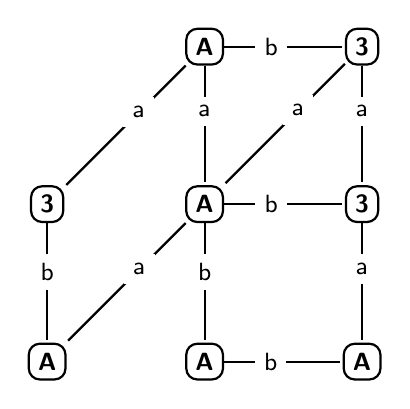
\begin{tikzpicture}[shorten >=1pt,auto,node distance=2cm,
                    thick,main node/.style={rounded corners,draw,font=\sffamily\small\bfseries}]

  \node[main node] (1) {A};
  \node[main node] (2) [right of=1] {3}; 
  \node[main node] (4) [below of =1] {A};
  \node[main node] (3) [left of=4] {3};
     \node[main node] (5) [below of=2] {3};
    \node[main node] (6) [below of=3] {A};
    \node[main node] (7) [below of=4] {A};
\node[main node] (8) [below of=5] {A};
  \path[every node/.style={font=\sffamily\small}]
    (1) edge[] node [minimum width = 1em, fill = white,pos=.25,right] {b} (2)
        edge[] node[minimum width = 1em, fill = white,pos=.25,below left] {a} (3)
        edge[] node[minimum width = 1em, fill = white,pos=.25,below] {a} (4)
    (2) edge[] node [minimum width = 1em, fill = white,pos=.25,below left] {a} (4)
        edge node [minimum width = 1em, fill = white,pos=.25,below] {a} (5)
    (3) edge[] node [minimum width = 1em, fill = white,pos=.25,below] {b} (6)
    (4) edge node [minimum width = 1em, fill = white,pos=.25,below] {b} (7)
    	edge[] node [minimum width = 1em, fill = white,pos=.25,below left] {a} (6) 
    	edge node [minimum width = 1em, fill = white,pos=.25,right] {b} (5) 
    (5) edge node [minimum width = 1em, fill = white,pos=.25,below] {a} (8)
    (7) edge node [minimum width = 1em, fill = white,pos=.25,right] {b} (8);	   
\end{tikzpicture}
\\\textbf{Step 4}
\end{minipage}\\
\hfill \vspace{5mm}\hfill \\
\begin{minipage}{.4\textwidth}
	\centering
	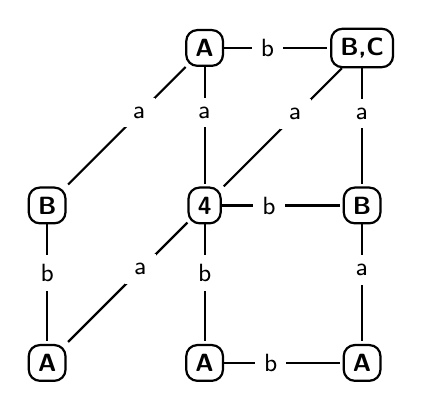
\begin{tikzpicture}[shorten >=1pt,auto,node distance=2cm,
                    thick,main node/.style={rounded corners,draw,font=\sffamily\small\bfseries}]

  \node[main node] (1) {A};
  \node[main node] (2) [right of=1] {B,C}; 
  \node[main node] (4) [below of =1] {4};
  \node[main node] (3) [left of=4] {B};
     \node[main node] (5) [below of=2] {B};
    \node[main node] (6) [below of=3] {A};
    \node[main node] (7) [below of=4] {A};
\node[main node] (8) [below of=5] {A};
  \path[every node/.style={font=\sffamily\small}]
    (1) edge[] node [minimum width = 1em, fill = white,pos=.25,right] {b} (2)
        edge[] node[minimum width = 1em, fill = white,pos=.25,below left] {a} (3)
        edge[] node[minimum width = 1em, fill = white,pos=.25,below] {a} (4)
    (2) edge[] node [minimum width = 1em, fill = white,pos=.25,below left] {a} (4)
        edge node [minimum width = 1em, fill = white,pos=.25,below] {a} (5)
    (3) edge[] node [minimum width = 1em, fill = white,pos=.25,below] {b} (6)
    (4) edge node [minimum width = 1em, fill = white,pos=.25,below] {b} (7)
    	edge[] node [minimum width = 1em, fill = white,pos=.25,below left] {a} (6) 
    	edge node [minimum width = 1em, fill = white,pos=.25,right] {b} (5) 
    (5) edge node [minimum width = 1em, fill = white,pos=.25,below] {a} (8)
    (7) edge node [minimum width = 1em, fill = white,pos=.25,right] {b} (8);	   
\end{tikzpicture}
\\\textbf{Step 5}
\end{minipage}
\begin{minipage}{.4\textwidth}
	\centering
	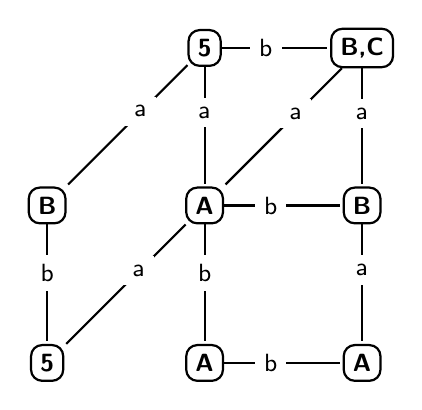
\begin{tikzpicture}[shorten >=1pt,auto,node distance=2cm,
                    thick,main node/.style={rounded corners,draw,font=\sffamily\small\bfseries}]

  \node[main node] (1) {5};
  \node[main node] (2) [right of=1] {B,C}; 
  \node[main node] (4) [below of =1] {A};
  \node[main node] (3) [left of=4] {B};
     \node[main node] (5) [below of=2] {B};
    \node[main node] (6) [below of=3] {5};
    \node[main node] (7) [below of=4] {A};
\node[main node] (8) [below of=5] {A};
  \path[every node/.style={font=\sffamily\small}]
    (1) edge[] node [minimum width = 1em, fill = white,pos=.25,right] {b} (2)
        edge[] node[minimum width = 1em, fill = white,pos=.25,below left] {a} (3)
        edge[] node[minimum width = 1em, fill = white,pos=.25,below] {a} (4)
    (2) edge[] node [minimum width = 1em, fill = white,pos=.25,below left] {a} (4)
        edge node [minimum width = 1em, fill = white,pos=.25,below] {a} (5)
    (3) edge[] node [minimum width = 1em, fill = white,pos=.25,below] {b} (6)
    (4) edge node [minimum width = 1em, fill = white,pos=.25,below] {b} (7)
    	edge[] node [minimum width = 1em, fill = white,pos=.25,below left] {a} (6) 
    	edge node [minimum width = 1em, fill = white,pos=.25,right] {b} (5) 
    (5) edge node [minimum width = 1em, fill = white,pos=.25,below] {a} (8)
    (7) edge node [minimum width = 1em, fill = white,pos=.25,right] {b} (8);	   
\end{tikzpicture}
\\\textbf{Step 6}
\end{minipage}
\caption{Algorithm Data Graph Processing}
 \label{fig:workingdg}
\end{figure}
\par In the data graph, the singleton NEC's are given according to the label of the node. In step 2 and Step 3 the nodes are getting NEC 1 and NEC 2 because the nodes matches the node label. NEC 1 and NEC 2 has no children to check. In step 4 the nodes are getting NEC 3 if it has a child with NEC 1 by an edge label 'a'. Then in step 5 the nodes are getting NEC 4 if it has a child of NEC 2 by edge label 'a'. In the final step the NEC 5 is given for nodes with two children. Each step describes the candidate set for each of the NEC's. $CVS(NEC 1)$ has 5 nodes. $CVS(NEC 2)$ has 1 node. $CVS(NEC 3)$ has 3 nodes. Then a actual tree matching is done using these CVS. All the combination of CVS are tested to find all possibilities of matching the tree in data graph. After that the non tree edges are checked.
\section{Inferences}
\hspace{10mm}The parallel version needs to store the mapped NEC for each node in the data graph. This is asking for a space of $O(n*N(q))$ where $n$ is number of nodes in data graph and $N(q)$ is number of  NEC in query graph. The time taken for executing complete graphs on various test scenarios are given below. These results are obtained on a NVIDIA CUDA supported GPU with 580 MHz speed. Stage 1 is the NEC finding on Query Graph. Stage 2 is the CVS finding. Stage 3 is the matching.$100n1000e$ means 100 nodes and 1000 edges. 

\begin{figure}[h]
 \centering
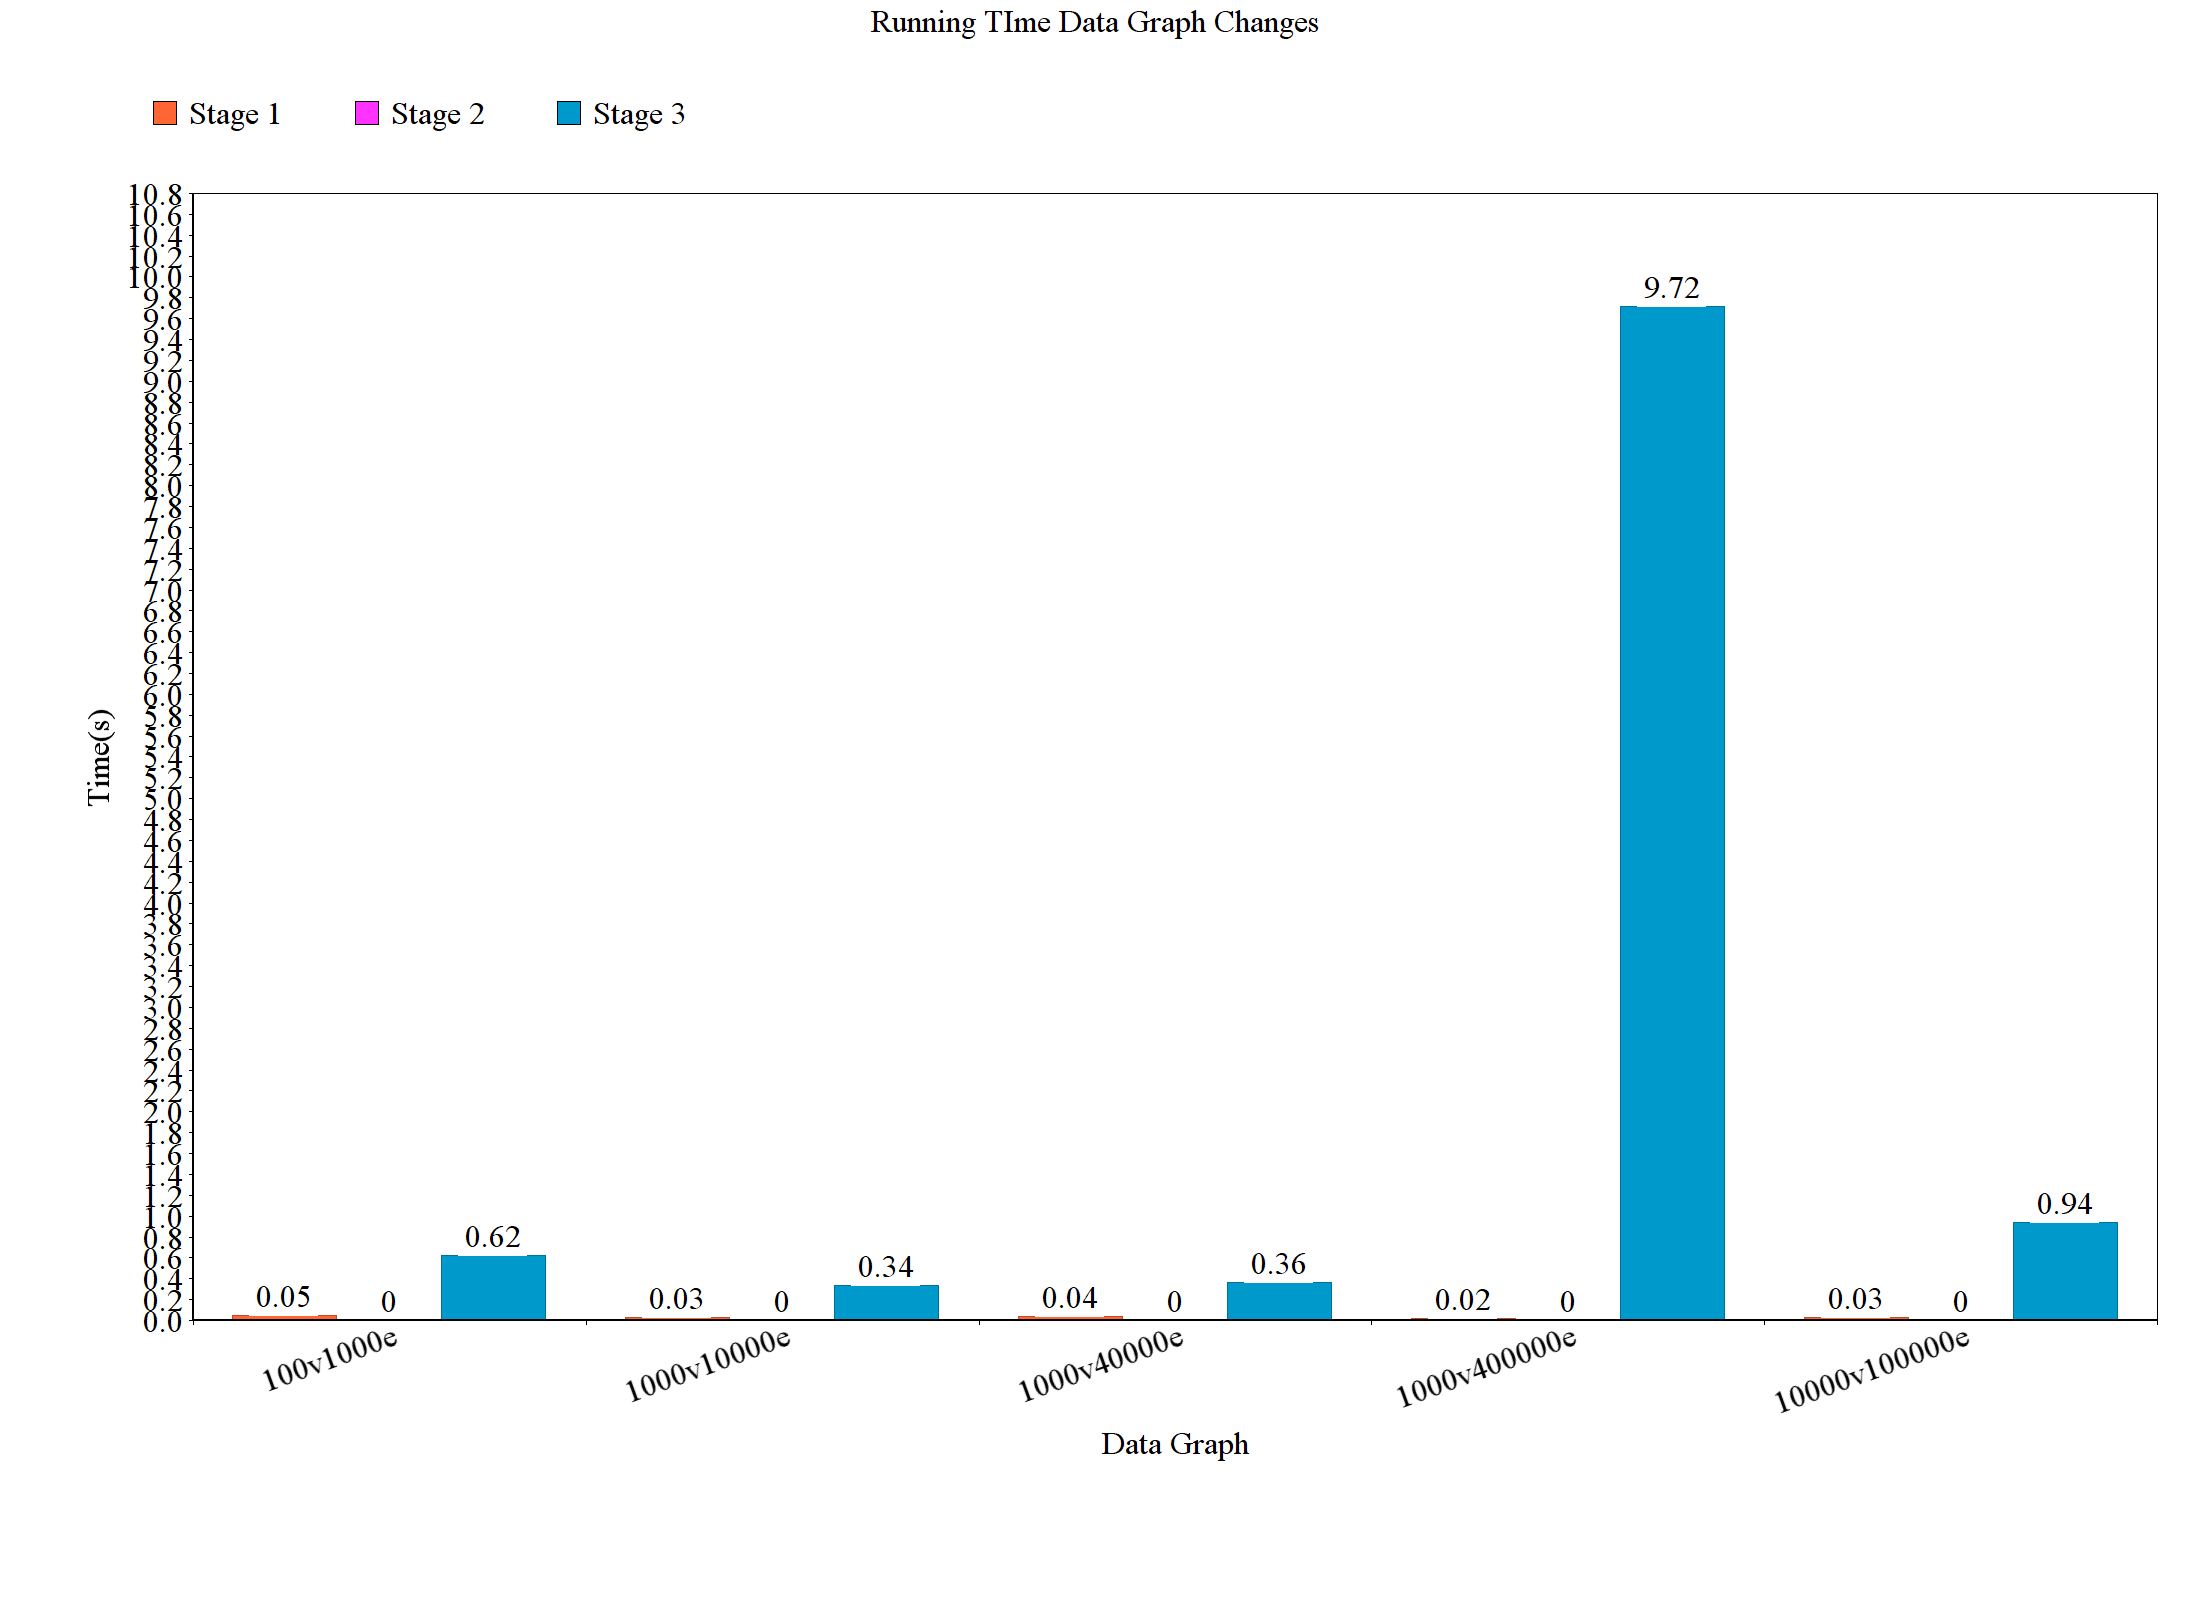
\includegraphics[width=.5\textwidth]{Dchange.png}
 \caption{Data Graph Size Changes}
 \label{fig:dchange}
\end{figure}
\hspace{10mm} When the data graph size changes the running times increases rapidly. The running time is depending on the density of the graph. If the size of the data graph increases and the density remains same, the running time doesn't show a spike. Fourth group shows a spike because of the huge density change from the other graphs. When the density changes the number of successful matching also increases causing the Stage 3(matching) to run more. \\
\begin{figure}[h!]
 \centering
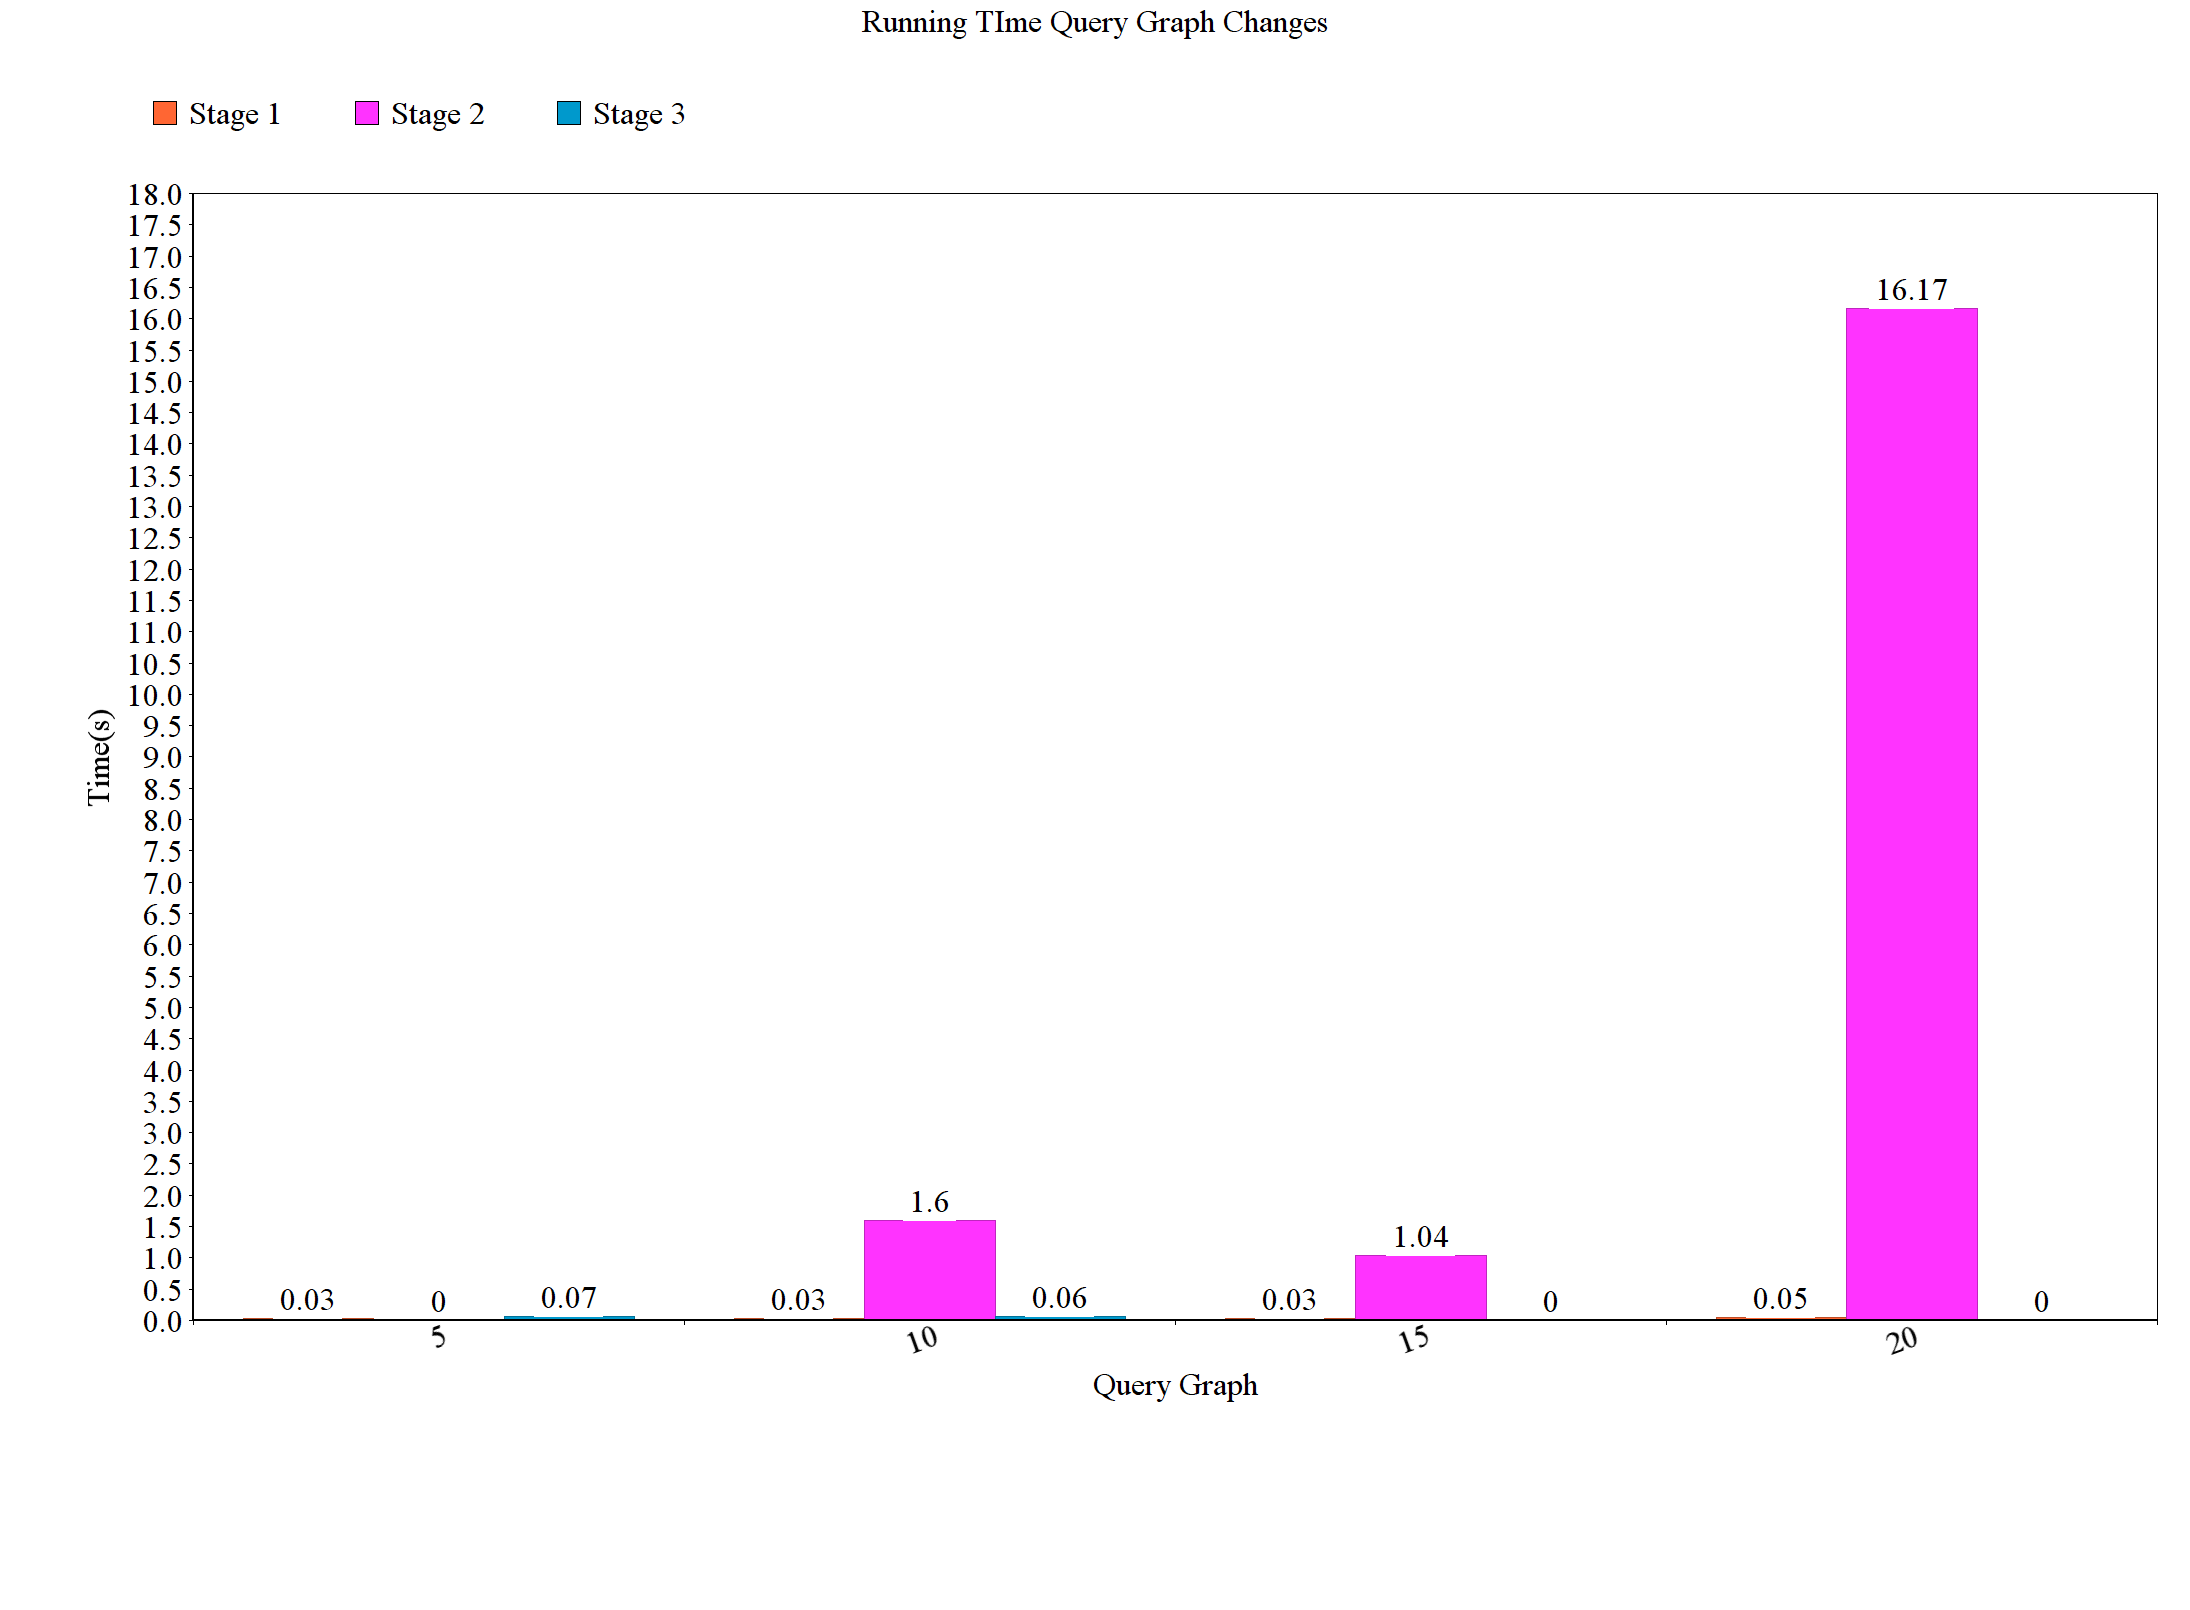
\includegraphics[width=.5\textwidth]{Qchange.png}
 \caption{Query Graph Size Changes}
 \label{fig:qchange}
\end{figure}
\hspace{10mm} When the query graph size changes the overall time increases. But the processing in Stage 2 is increased. The Stage 2 depends on the number of NEC. The NEC count will increase if the number of nodes in query graph increases. The Stage 3 is getting zero because the CVS becomes null set. No candidate would have been found for higher level nodes. This will help to not run Stage 3 making the time zero.\\
\begin{figure}[h!]
 \centering
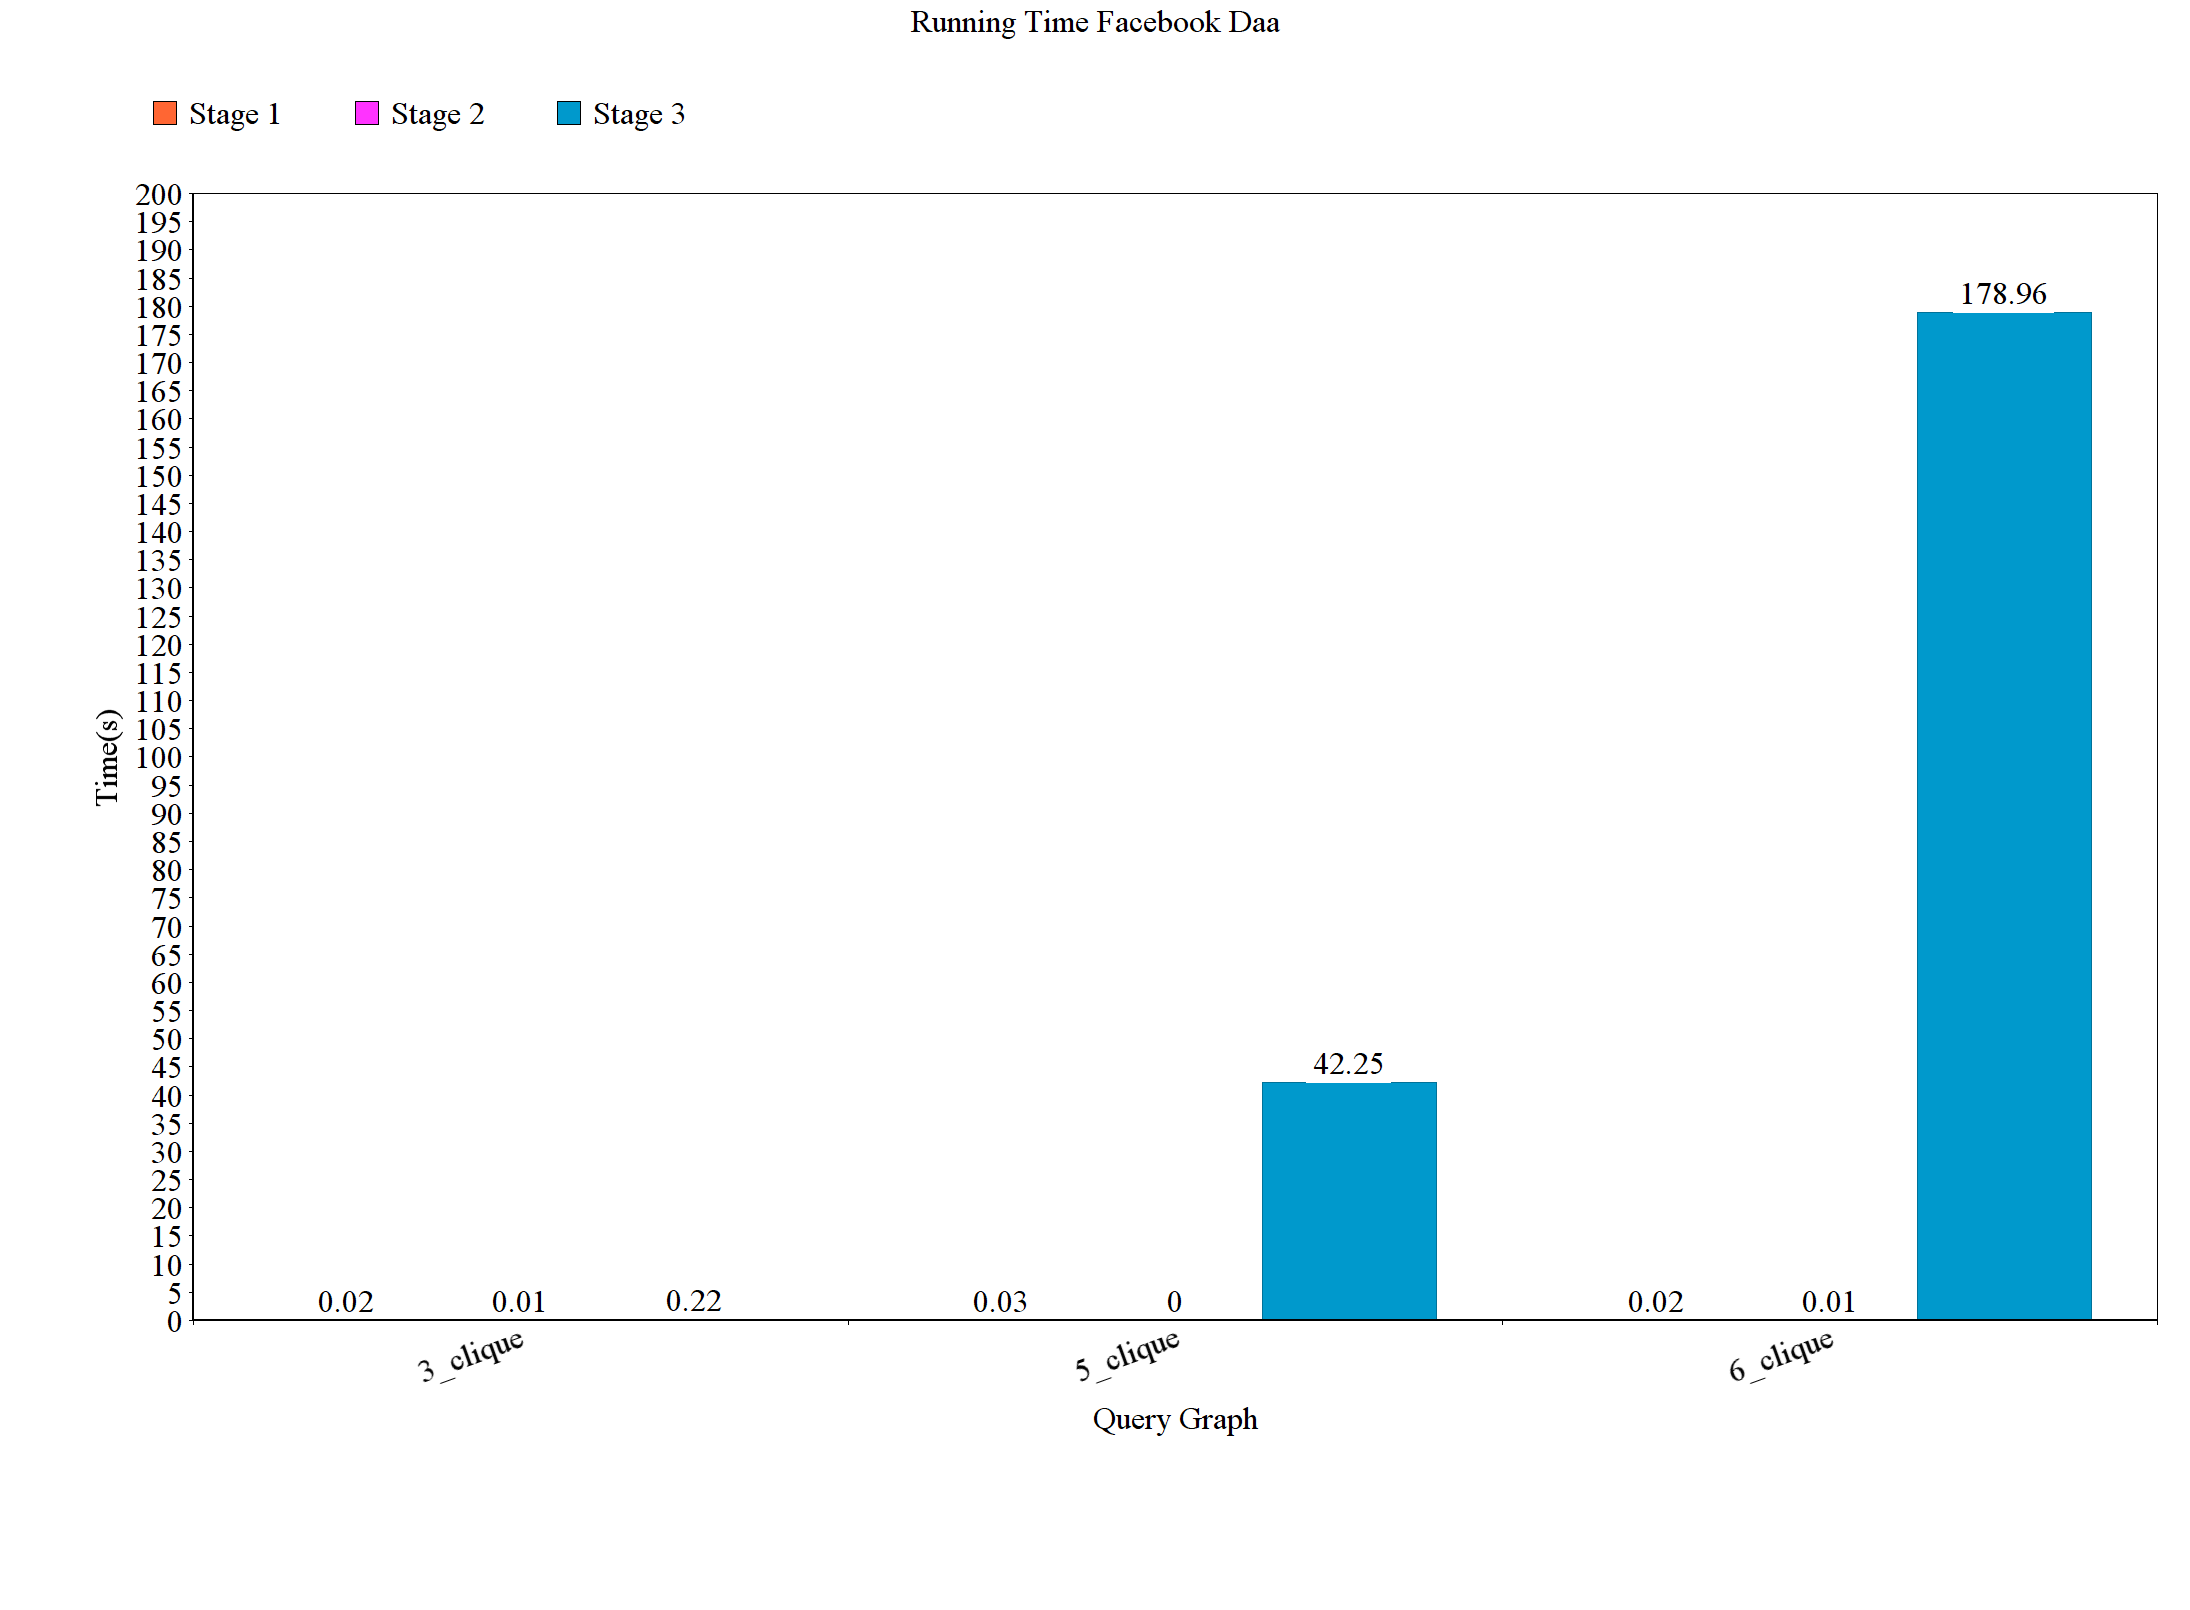
\includegraphics[width=.5\textwidth]{fb.png}
 \caption{Facebook network}
 \label{fig:fb}
\end{figure}
\hspace{10mm} Facebook Data is having 4039 nodes and 88234 edges making it a slightly dense network. Even if the final number of cliques of size 5 and 6 are in the range of number of triangle. Number of possible checks requires increases. Each node addition will cause to calculate almost 100(from CVS size) more possibilities. The false candidates are not easy to remove since the graph is fairly dense.\\
\begin{figure}[h!]
 \centering
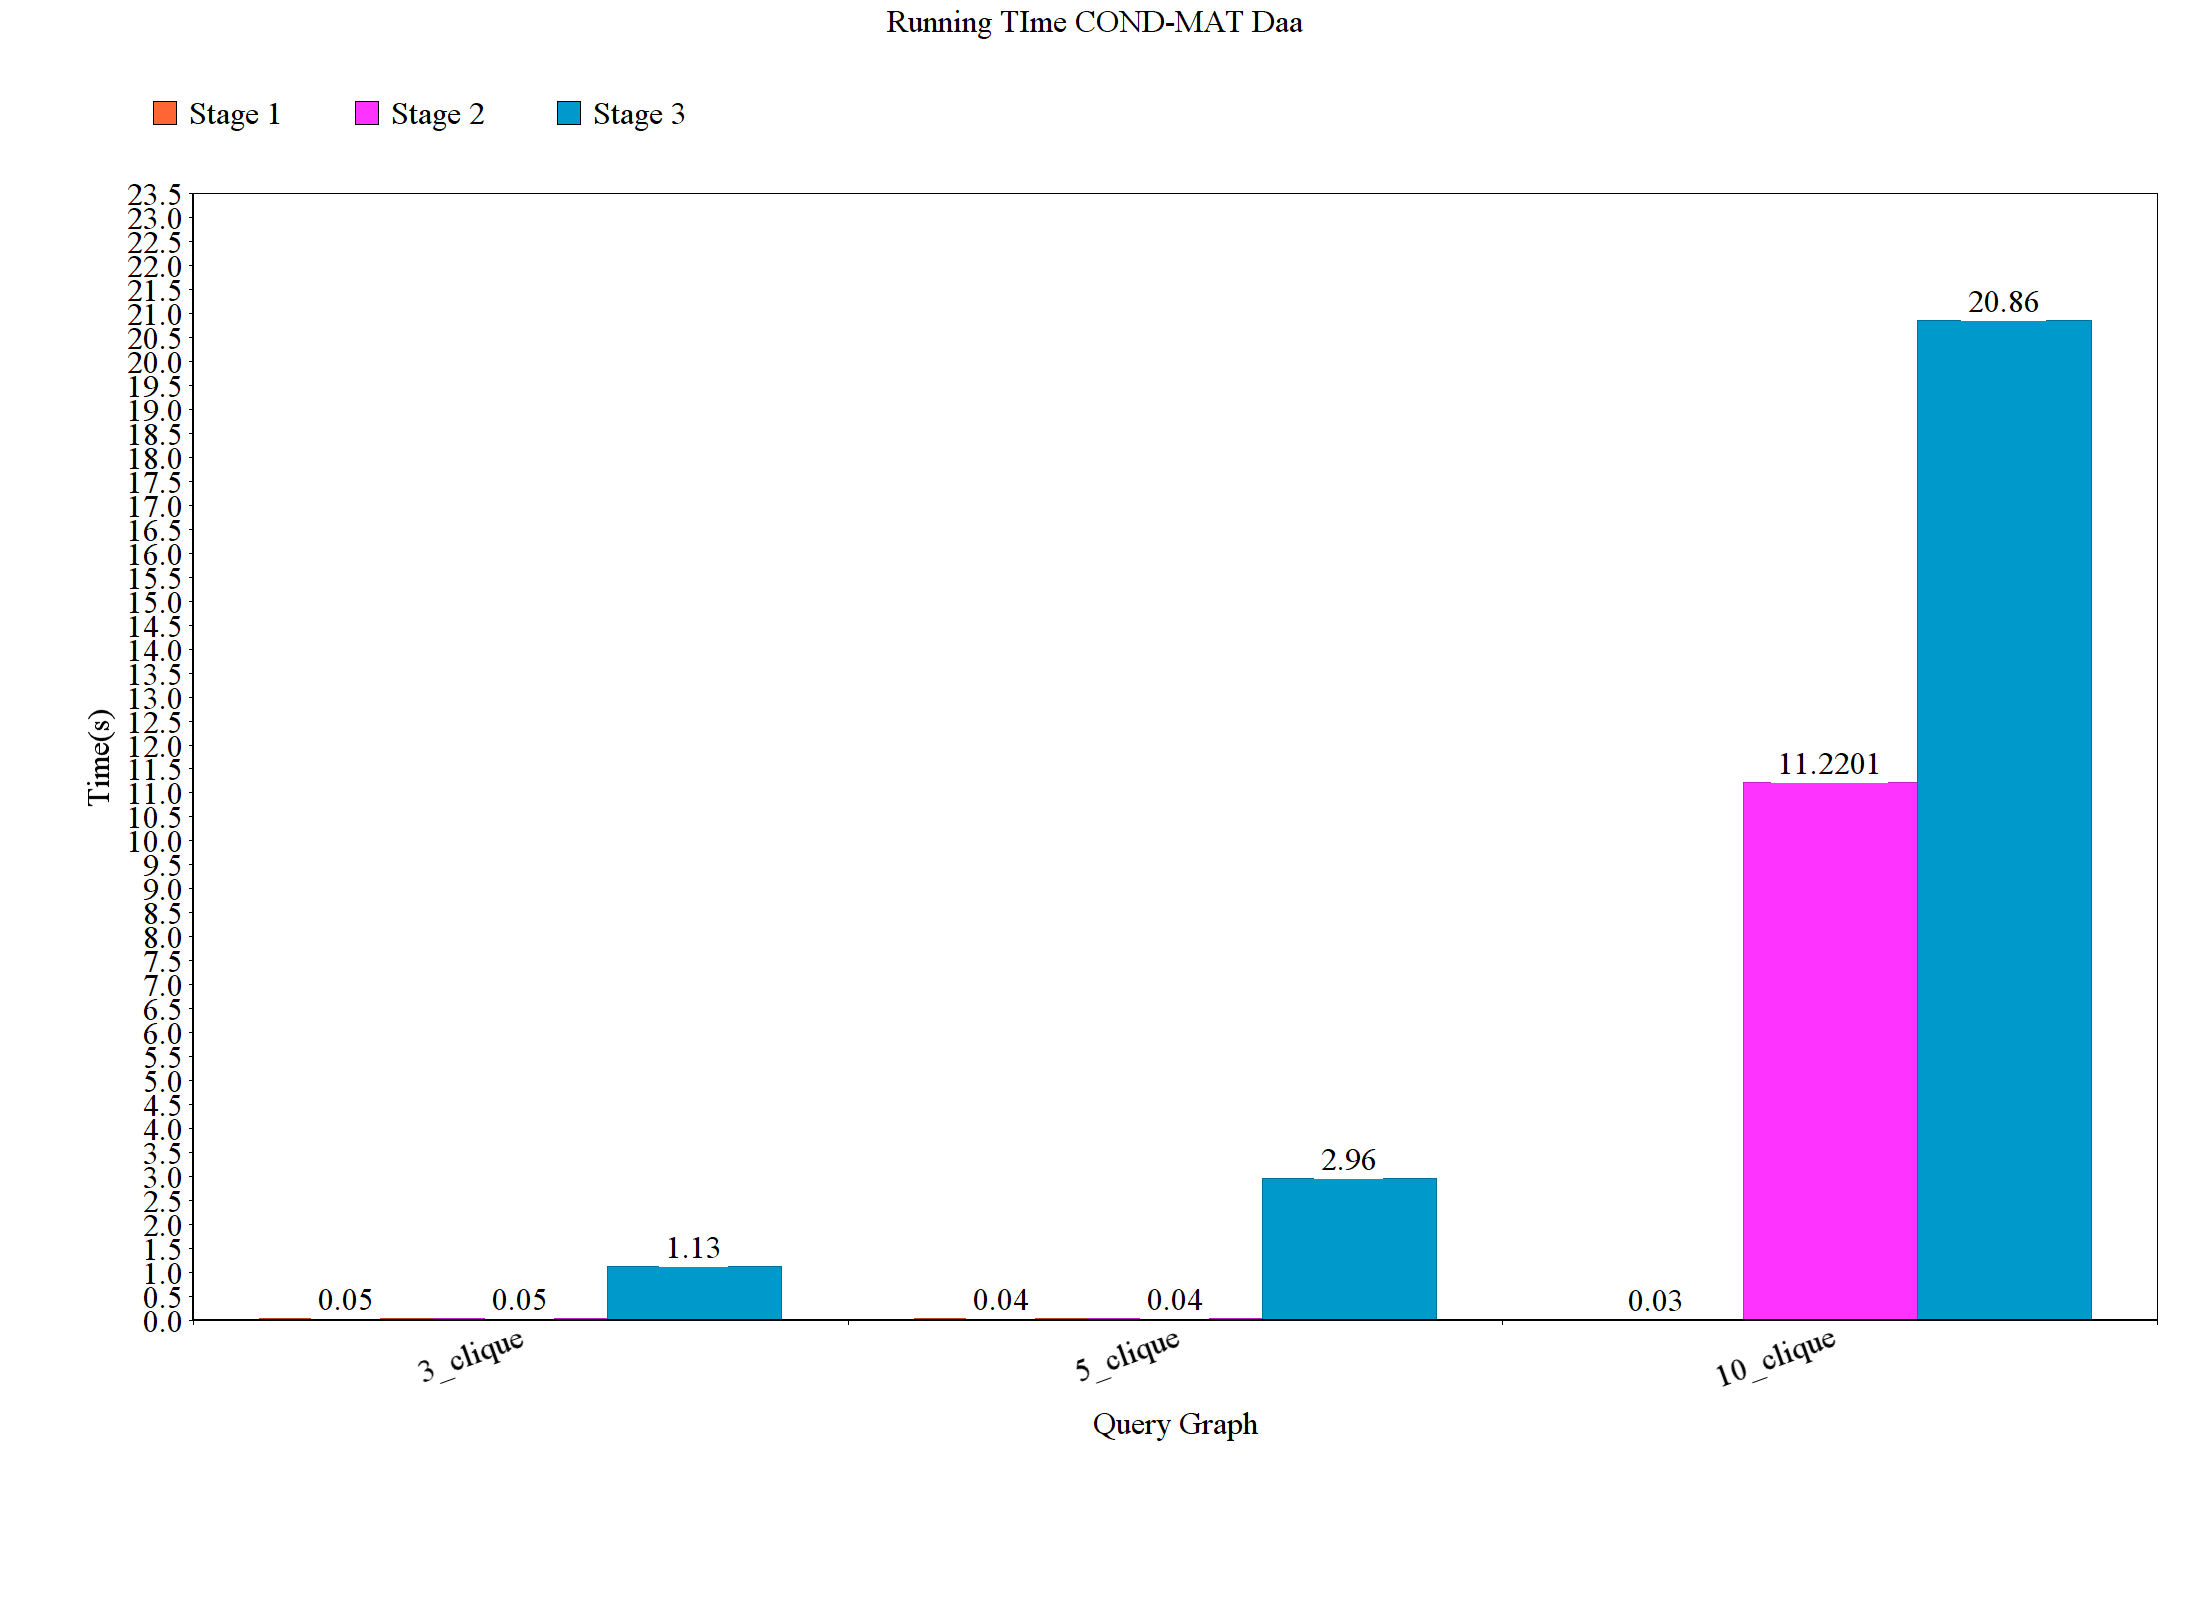
\includegraphics[width=.5\textwidth]{CA.png}
 \caption{Condense Matter collaboration network}
 \label{fig:ca}
\end{figure}
\hspace{10mm}Condense Matter collaboration network Dataset is having 23133 nodes and 93497 edges. The graph is slightly sparse. The number of higher node cliques are less and the possibilities of finding them is also getting reduced due to the sparsity of the graph. The increase in time is not that steep because of the low density.
\section{Failed Approach}
	\hspace{10mm}We tried to make the the NEC numbering more informative by using primes and composites. A prime will be assigned to a class if that graph has no other embedding of any previous graphs we came across. If it has the embedding we give product of the prime numbers of the embedding. This method helps to know that if the NEC has a composite number it has some smaller graphs embedded in it. So we won't be needed to  search the sub-graphs in this node.\\
\hspace{10mm}	It actually captures all sub-graphs at the root. See the figure \ref{fig:NEC}.\\
	\begin{figure}[h]
 \centering
%\centering
\begin{minipage}{.6\textwidth}
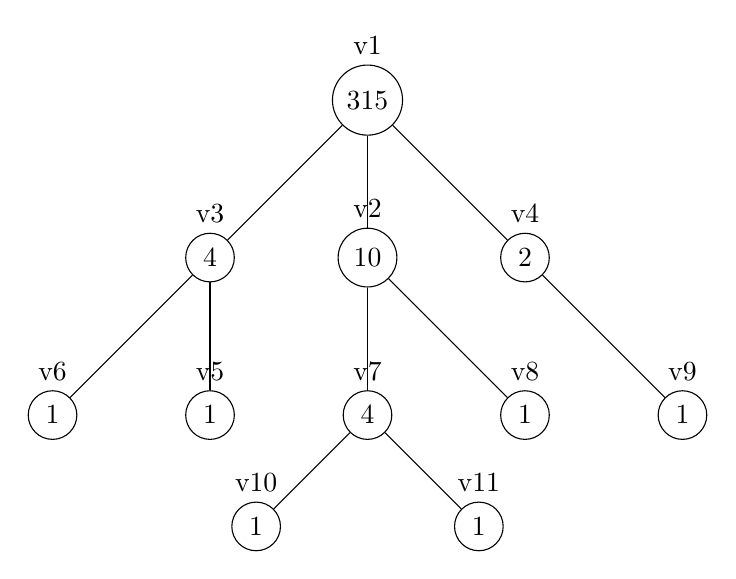
\begin{tikzpicture}[node distance=2cm]
\node[circle,draw,label=v1] (1)[]{315};
\node[circle,draw,label=v2] (3)[below of=1]{10};
\node[circle,draw,label=v3] (2)[left of=3]{4};
\node[circle,draw,label=v4] (4)[ right of=3]{2};
\node[circle,draw,label=v5] (5)[below of=2]{1};
\node[circle,draw,label=v6] (6)[left of=5]{1};
\node[circle,draw,label=v7] (7)[below of=3]{4};
\node[circle,draw,label=v8] (8)[right of=7]{1};
\node[circle,draw,label=v9] (9)[right of=8]{1};
\node[circle,draw,label=v10] (10)[below left of=7]{1};
\node[circle,draw,label=v11] (11)[below right of=7]{1};
\path
	(1) edge node{} (2)
		 edge node{} (3)
		 edge node{} (4)
	(2) edge node{} (5)
		edge node{} (6)
	(3) edge node{} (7)
		edge node{} (8)
	(4) edge node{} (9)
	(7) edge node{} (10)
		edge node{} (11);	
\end{tikzpicture}
\end{minipage}
\begin{minipage}{.2\textwidth}
\centering
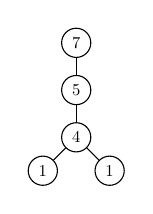
\begin{tikzpicture}[scale=0.1,every node/.style={scale=0.6}]
\node[circle,draw] (5)[]{7};
\node[circle,draw] (1)[below of=5]{5};
\node[circle,draw] (2)[below of=1]{4};
\node[circle,draw] (3)[below left of=2]{1};
\node[circle,draw] (4)[below right of=2]{1};
\path
	(5) edge node{} (1)
	(1) edge node{} (2)
	(2)	 edge node{} (3)
		 edge node{} (4);
\end{tikzpicture}\\Intermediate graph \hfill \\
\begin{tikzpicture}[scale=0.1,every node/.style={scale=0.6}]

\node[circle,draw] (1)[]{3};
\node[circle,draw] (2)[below of=1]{2};
\node[circle,draw] (3)[below of=2]{1};
\path
	(5) edge node{} (1)
	(1) edge node{} (2)
	(2)	 edge node{} (3);
\end{tikzpicture}
\\Intermediate Graph
\end{minipage}
 \caption{NEC based on primes}
 \label{fig:NEC}
\end{figure}
\hspace{10mm}  $v4$ is getting 2 since it has only one child $1$. $v7$ and $v3$ gets 4 since it has two same sub-graphs(sub-graph $2$) inside them. $v2$ is getting 10 since it has sub-graph $2$ and $5$ (see the numbering shown on right). Similarly $v1$ has two $3$s($v2$ contributes one $3$) ,one $7$ and one $5$.

 \hspace{10mm}	But this was not effective.When we consider the data graph we will need to store only one integer the product of all the graphs inside that node. The first problem we faced was the value of composite number can go beyond the long integer limit. So we tried only storing primes. But that also didn't make much difference. By our propagation algorithm in Data Graph, we start by giving id $1$ to all nodes in the data graph in the first iteration. In the second iteration every node will get id $2$ since every node will have a child of id $1$. Then in third every node will get $3$ and so on. So every node gets every id present in query graph.
 
 \hspace{10mm} It only helped as in knowing whether there exist a path of length matching the largest length path in query graph. This will lead to all nodes becoming a candidate for the final search we atleast one graph existed in the connected component. So it is not making the CVS tight.
	